% file: ThePhysicsOfInterstellar.tex
% AdS/CFT and Interstellar
% 
% github        : ernestyalumni
% linkedin      : ernestyalumni 
% wordpress.com : ernestyalumni
%
% This code is open-source, governed by the Creative Common license.  Use of this code is governed by the Caltech Honor Code: ``No member of the Caltech community shall take unfair advantage of any other member of the Caltech community.'' 
% 

\documentclass{beamer}

% cf. https://tex.stackexchange.com/questions/40253/how-to-strike-through-obliquely-e-g-to-indicate-cancellation
\usepackage{cancel}

% cf. https://tex.stackexchange.com/questions/38352/resize-scale-equation-in-beamer
\usepackage{graphicx}% http;//ctan.org/pkg/graphicx


\usetheme{default}

% cf. https://tex.stackexchange.com/questions/79420/changing-font-style-using-beamer
\usefonttheme{structuresmallcapsserif} % using non standard fonts for beamer
\usefonttheme{serif} % default family is serif

\title{
	\centering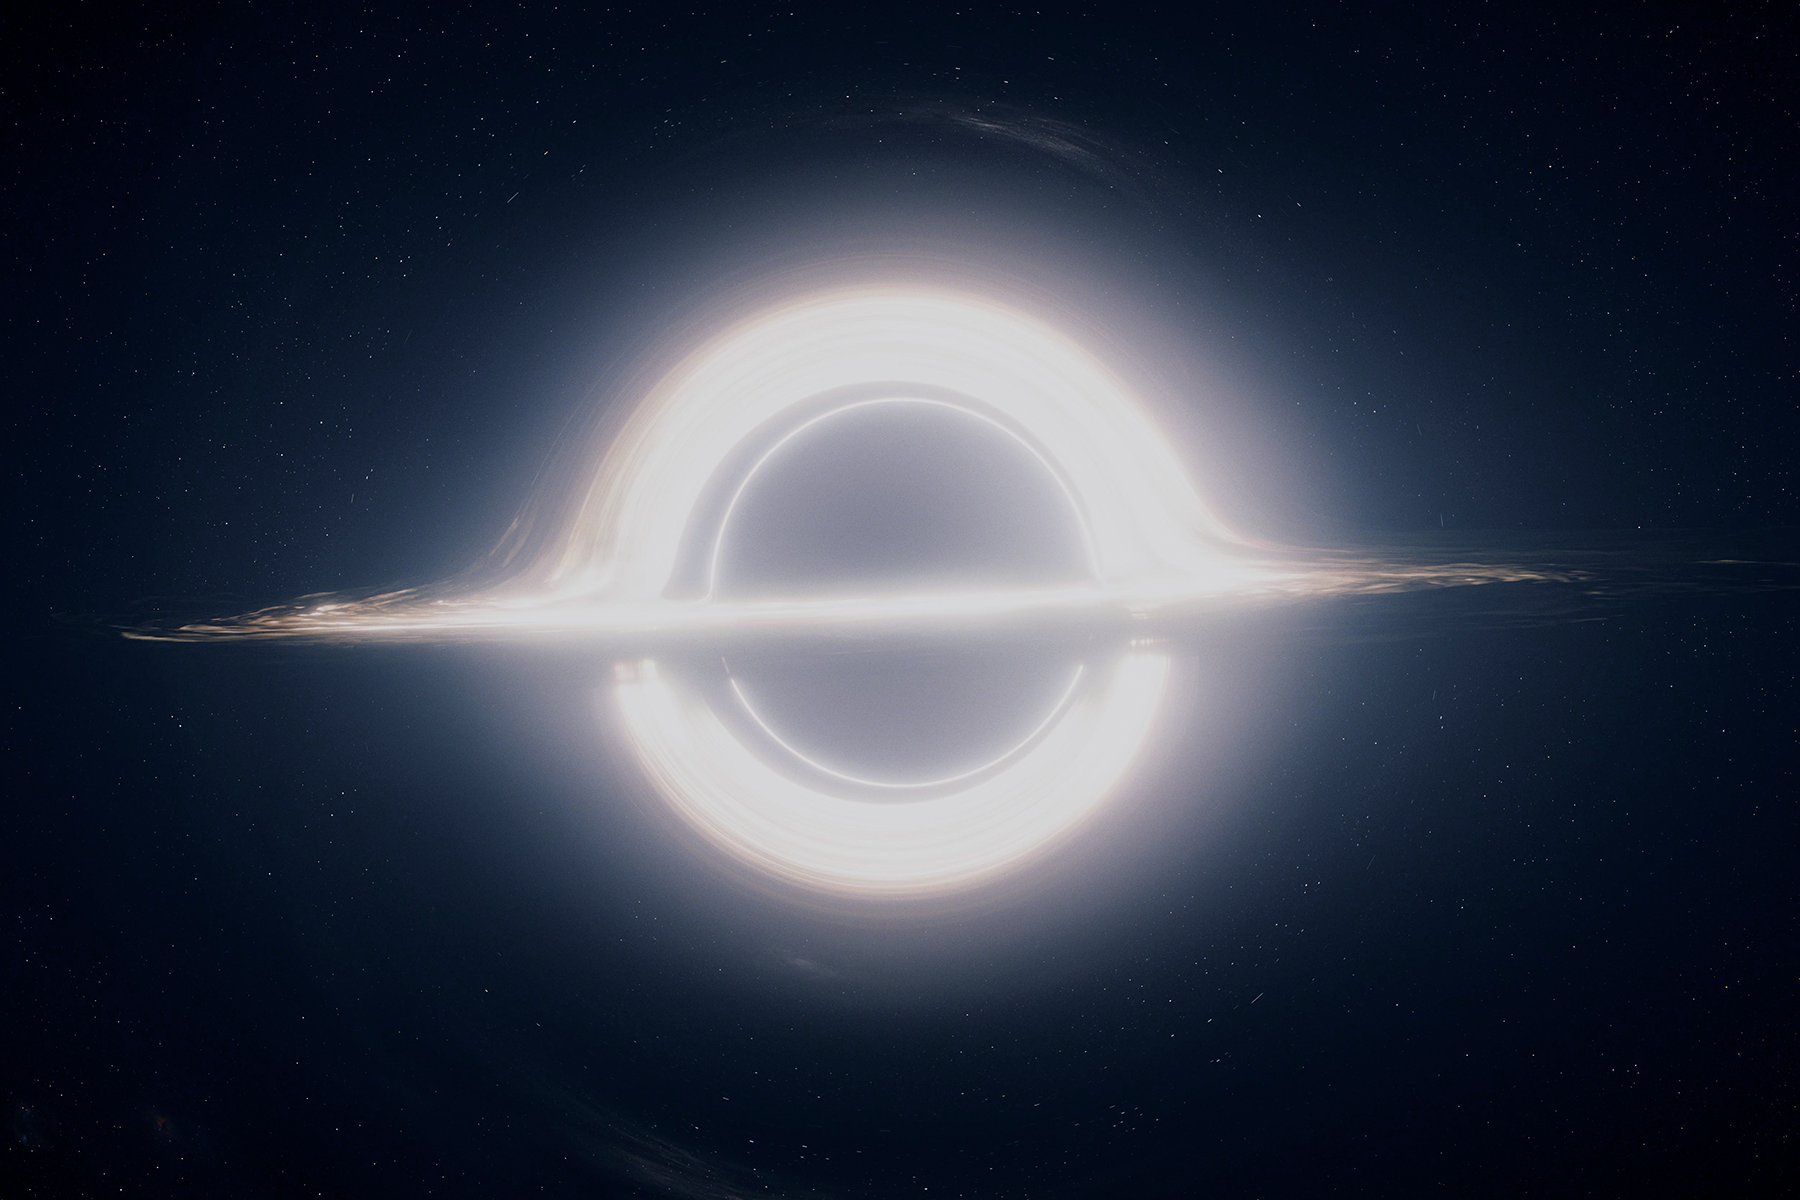
\includegraphics[width=0.85\textwidth]{images/ut_interstellarOpener_f.png}\\	
	The Physics of Interstellar
}
\author{Ernest Yeung}

\begin{document}
	% Title page frame.
	\begin{frame}
		\titlepage
	\end{frame}
	\begin{frame}{Gravitational lensing of spinning (Kerr) black holes}
		\begin{figure}
			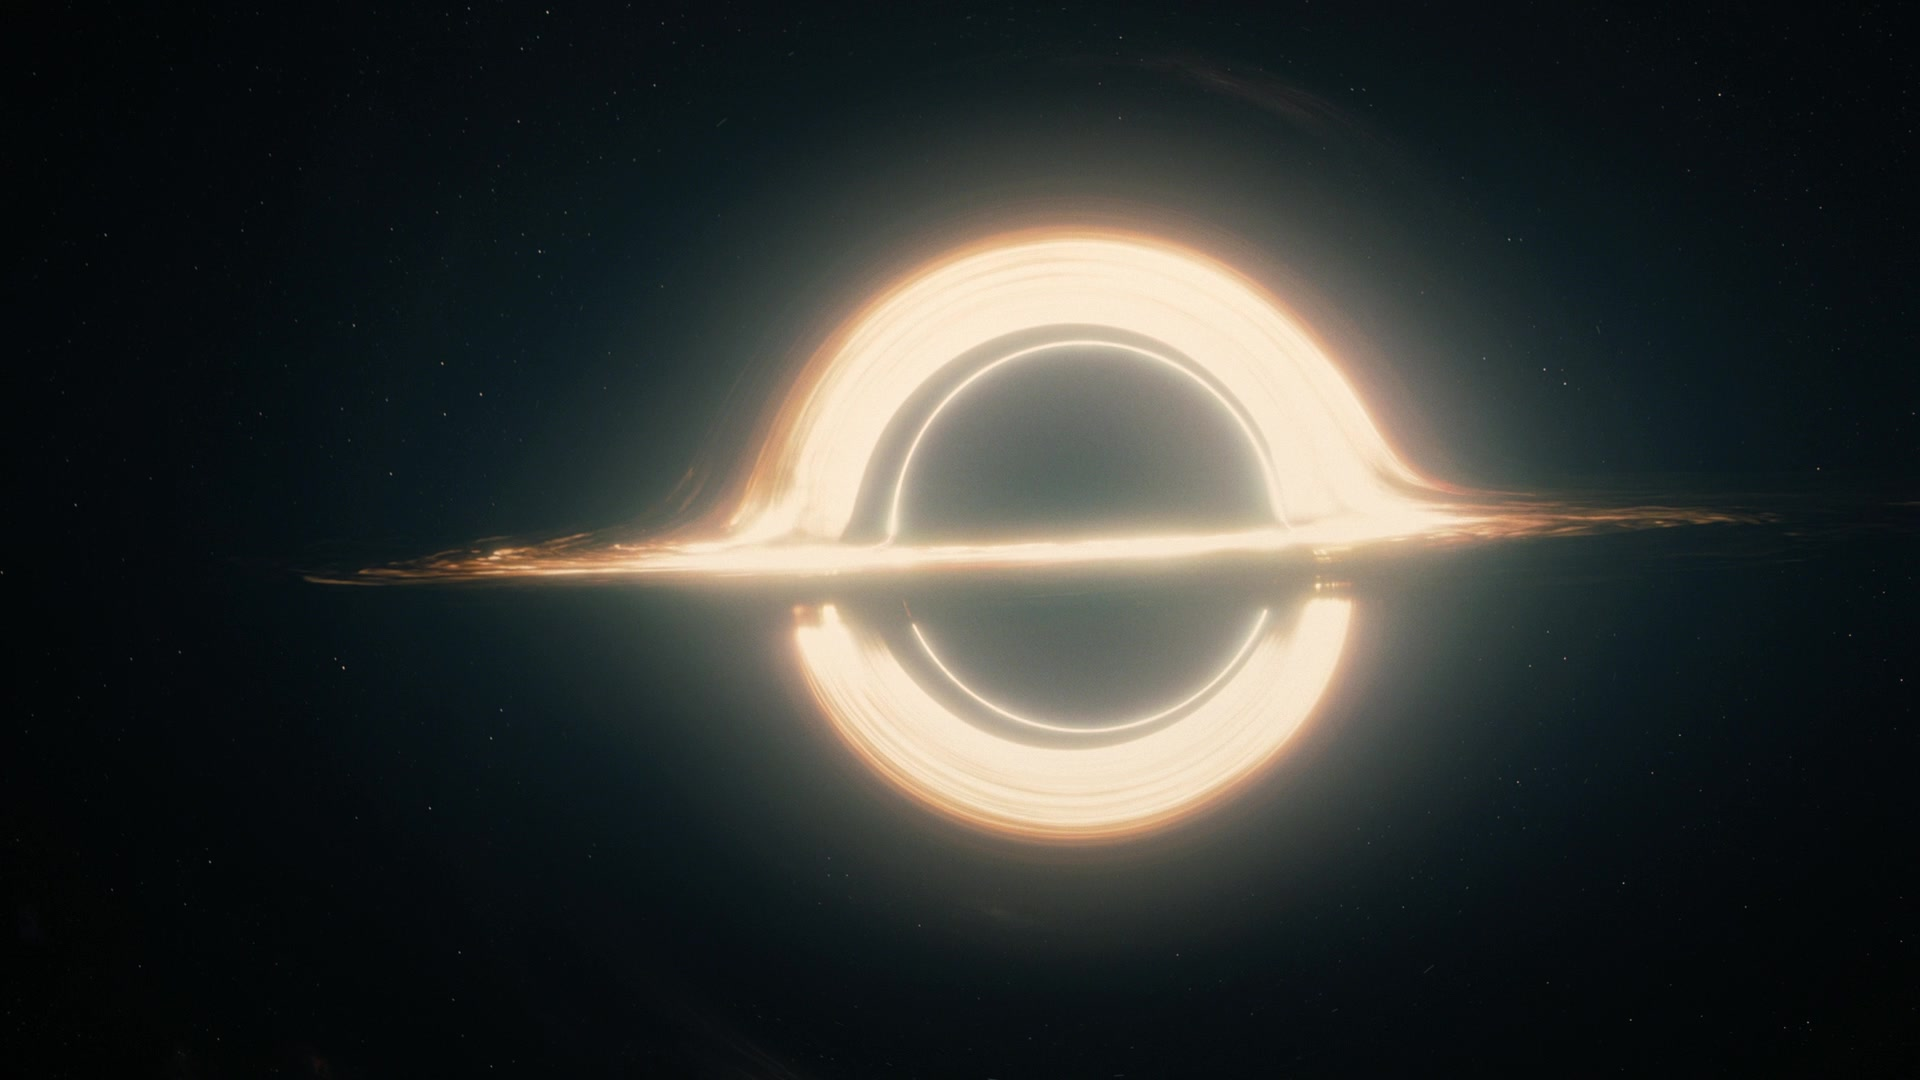
\includegraphics[width=\textwidth]{images/1200899.jpg}
		\end{figure}
	\end{frame}
	\begin{frame}
		Spoiler alert!
	\end{frame}
	\begin{frame}{"...but they constructed this 3-dim. (dimensional) space inside their 5-dim. reality to allow you to understand it..."}
			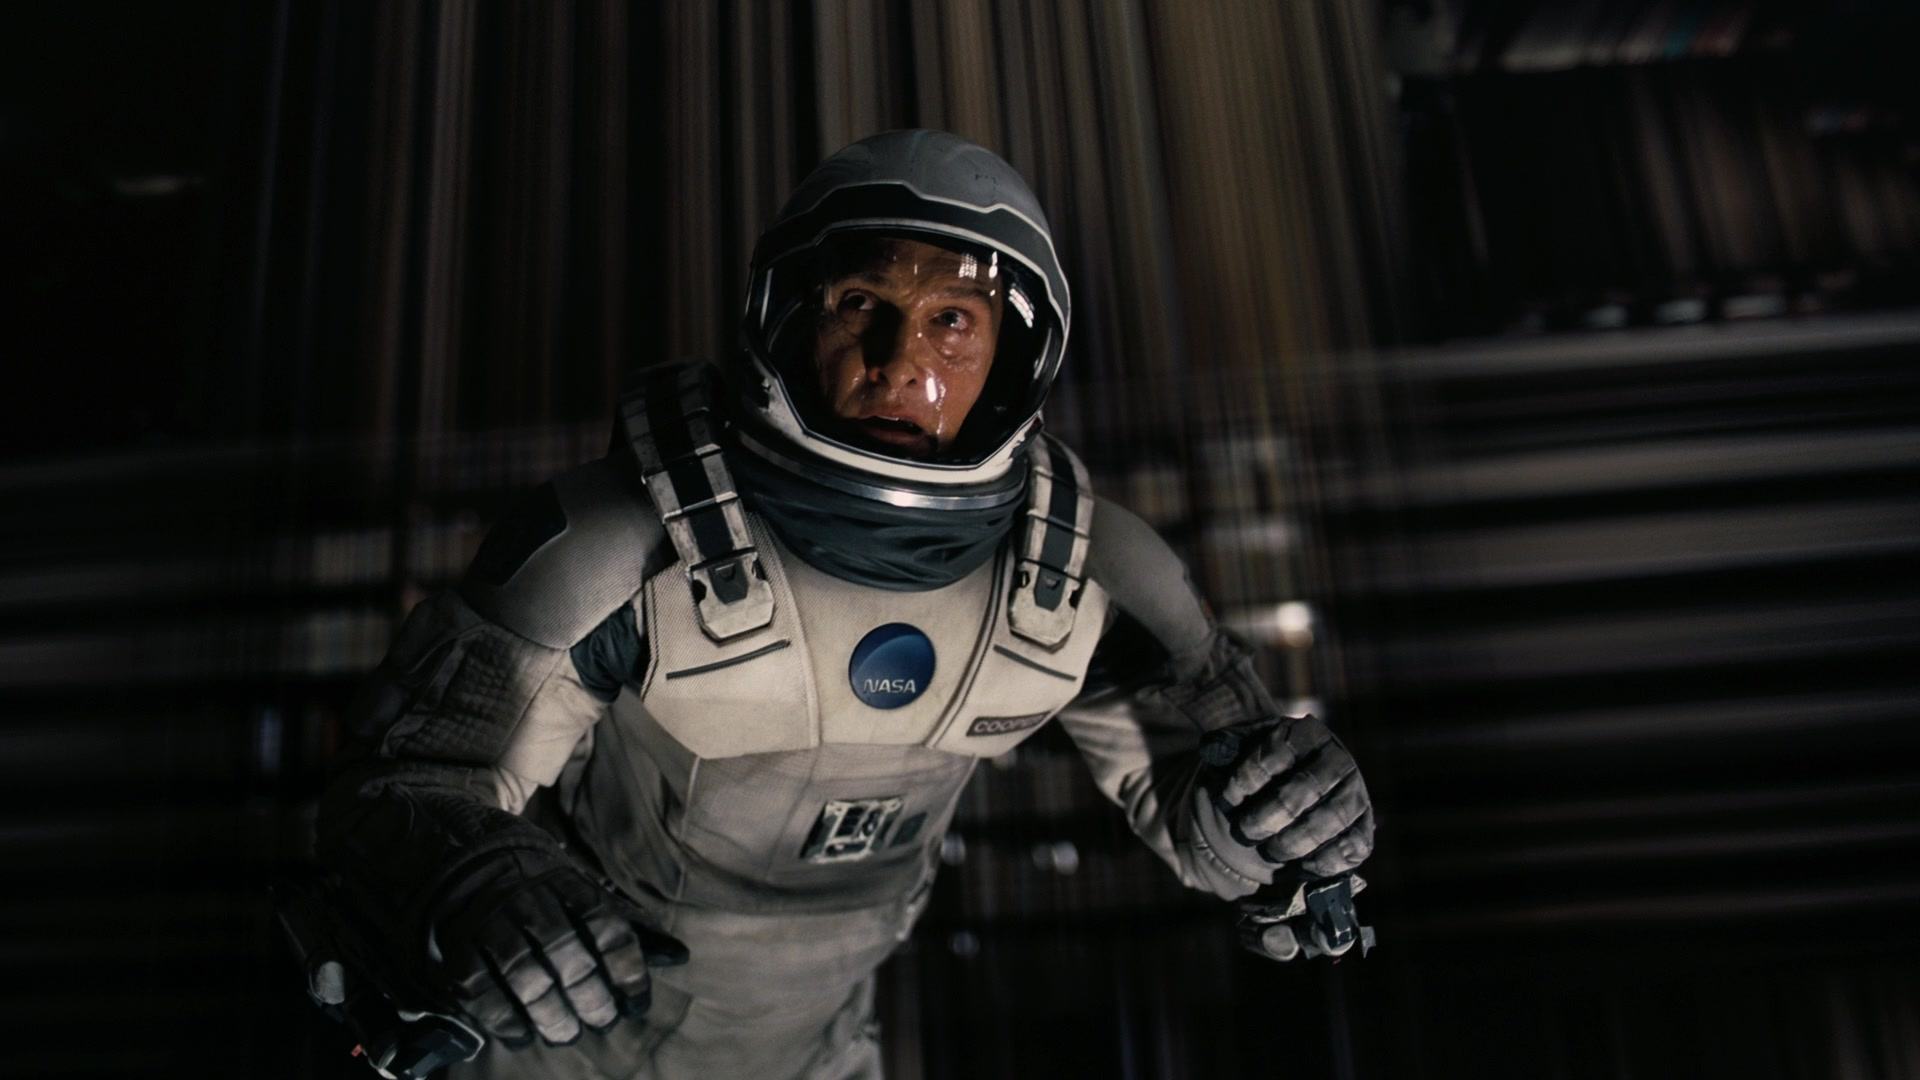
\includegraphics[width=\textwidth]{images/1201308.jpg}		
	\end{frame}
	\begin{frame}{Einstein's Theory of General Relativity}
		\begin{equation*}
			R_{ab} - \frac{1}{2} g_{ab} R = 8\pi G_N T_{ab}
		\end{equation*}
		\begin{equation*}
			S_{\text{Einstein-Hilbert}}[g] = \int_M \sqrt{-g} R
		\end{equation*}
	\end{frame}
	\begin{frame}{Metric $g$}
		\begin{columns}
			\begin{column}{0.5\textwidth}
				Minkowski metric (flat)
					\begin{equation*}
						g = -dt^2 + dx^2 + dy^2 + dz^2
					\end{equation*}
			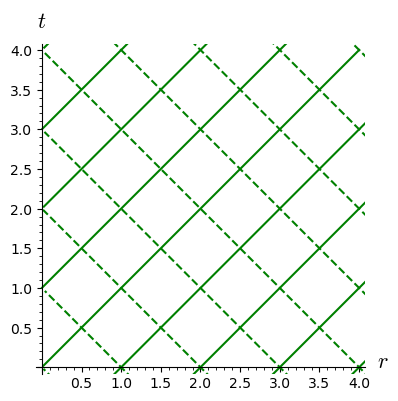
\includegraphics[width=0.4\textwidth]{images/conformal_Minkowskiindex.png}						
			\end{column}
			\begin{column}{0.5\textwidth}  %%<--- here
				Schwarzschild (static, non-spinning black hole) metric
					\scalebox{0.5}{%
						$g = -d\tau^2 = -\left( 1 - \frac{r_s}{r} \right) dt^2 + \left( 1 -\frac{r_s}{r} \right)^{-1} dr^2 + r^2 (d\theta^2 + \sin^2{\theta} d\phi^2)$
				}
			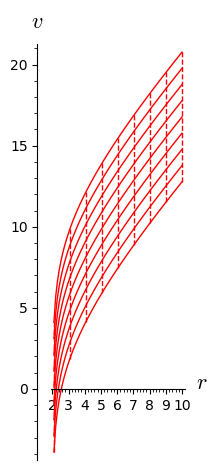
\includegraphics[width=0.4\textwidth]{images/SM_Schwarzschild_BoyerLindquistplotindex.png}						
			\end{column}
		\end{columns}
	\end{frame}
	\begin{frame}{Quantum Field Theory (The Standard Model)}
	The Standard Model
		\begin{equation*}
			\begin{aligned}
				\mathcal{L}_{fg} = & \frac{-1}{4} G^{\alpha}_{\mu \nu} G^{\alpha \mu \nu} - \frac{1}{4} W^{a\mu \nu} W^{a}_{\mu \nu} - \frac{1}{4} B_{\mu \nu} B^{\mu \nu} - \frac{g_3^2 \Theta_3}{64\pi^2} \epsilon_{\mu \nu \lambda \rho} G^{\alpha \mu \nu} G^{\alpha \lambda \rho} \\
& - \frac{g_2^2 \Theta_2}{64 \pi^2} \epsilon_{\mu \nu \lambda \rho} W^{a \mu \nu} W^{a\lambda \rho } - \frac{g_1^2 \Theta_1}{64 \pi^2 } \epsilon_{\mu \nu \lambda \rho} B^{\mu \nu} B^{\lambda \rho} - \frac{1}{2} \overline{L}_m \cancel{D} L_m \\ 
& - \frac{1}{2} \overline{E}_m \cancel{D} E_m - \frac{1}{2} \overline{Q}_m \cancel{D} Q_m - \frac{1}{2} \overline{U}_m \cancel{D} U_m - \frac{1}{2} \overline{D}_m \cancel{D} D_m
			\end{aligned}
		\end{equation*}
in which gauge field-strengths given by
\[
\begin{aligned}
G^{\alpha}_{\mu \nu} & = \partial_{\mu} G_{\nu}^{\alpha} - \partial_{\nu} G_{\mu}^{\alpha} + g_3 f^{\alpha}_{\, \, \beta \gamma} G_{\mu}^{\beta} G_{\nu}^{\gamma} \\
W^a_{\mu \nu} & = \partial_{\mu} W_{\nu}^a - \partial_{\nu} W^a_{\mu} + g_2 \epsilon_{abc} W^b_{\mu} W^c_{\nu} \\
B_{\mu \nu} & = \partial_{\mu} B_{\nu} - \partial_{\nu} B_{\mu}
\end{aligned}
\]
\[
\begin{gathered}
 + \mathcal{L}_{\text{Higgs}}
\end{gathered}
\]
	\end{frame}
\begin{frame}{Quantum Field Theory (Symmetry)}
Invariance of Lagrangian under symmetries
	\begin{equation*}
{\tiny		\begin{aligned}
			& \delta L_m = \left[ \left( \frac{-i}{2} \omega_1(x) + \frac{i}{2} \omega_2^a(x) \tau_a \right) P_L + \left( \frac{i}{2} \omega_1(x) - \frac{i}{2} \omega_2^a(x) \tau^*_a \right) P_R \right] L_m \\
			& \delta E_m = [ i\omega_1(x) P_L - i \omega_1(x) P_R ] E_m \\
			& \delta Q_m = \left[ \left( \frac{i}{6} \omega_1(x) + \frac{i}{2} \omega_2^a(x) \tau_a + \frac{i}{2} \omega_3^{\alpha}(x) \lambda_{\alpha} \right) P_L +  \right. \\
			& \phantom{\delta Q_m =} \left. + \left( -\frac{i}{6} \omega_1(x) - \frac{i}{2} \omega_2^a(x) \tau^*_a - \frac{i}{2} \omega_3^{\alpha}(x) \lambda_{\alpha}^* \right) P_R \right] Q_m \\
			& \delta U_m = \left[ \left( \frac{-2i}{3} \omega_1(x) - \frac{i}{2} \omega_3^{\alpha}(x) \lambda_{\alpha}^* \right) P_L + \left( \frac{2i}{3} \omega_1(x) _ \frac{i}{2} \omega_3^{\alpha}(x) \lambda_{\alpha} \right) P_R \right] U_m \\
			& \delta D_m = \left[ \left( \frac{i}{3} \omega_1(x) - \frac{i}{2} \omega_3^{\alpha}(x) \lambda_{\alpha}^* \right) P_L + \left( -\frac{i}{3} \omega_1(x) + \frac{i}{2} \omega_3^{\alpha}(x) \lambda_{\alpha} \right) P_R \right] D_m \\
			& \delta G_{\mu}^{\alpha} = \partial_{\mu} \omega_3^{\alpha}(x) - f^{\alpha}_{\beta \gamma} \omega_3^{\beta}(x) G_{\mu}^{\gamma} \\
			& \delta W_{\mu}^a = \partial_{\mu} \omega_2^a(x) - \epsilon^{abc} \omega_2^b(x) W_{\mu}^c \\
			& \delta B_{\mu} = \partial_{\mu} \omega_1(x)
		\end{aligned} }
	\end{equation*}

		Symmetry groups
		\begin{equation*}
{\small 			\begin{aligned}
				 SU_c(3) \times \quad & SU_L(2)  \times & U_Y(1) \\
				 \downarrow \quad & \downarrow & \downarrow \\
				 8 G_{\mu}^{\alpha} \quad & 3 W_{\mu}^a & B_{\mu} \\
				 \alpha = 1, \dots, 8 \quad & a = 1, 2, 3 & \\
			\end{aligned} \quad \quad \, \begin{aligned}
& U_{\text{em}} \\ 
& \downarrow \\
& \gamma
\end{aligned} }
		\end{equation*}

% Quantization
\end{frame}

\begin{frame}{Information, Entropy, and Black Holes}

Entropy

\[
\begin{gathered}
\begin{gathered}
\text{(Information Theory)} \\
H(X) := -\sum_{x \in X} p(x) \log_2{p(x)} 
\end{gathered} \\
\begin{aligned} 
 & \text{(Classical)} & \text{(Quantum)} \\
& S = - \sum p_i \ln{ p_i} & S = -\text{Tr}{ (\rho \ln{ \rho } )} \\
\end{aligned}
\end{gathered}
\]

Black hole entropy
\begin{equation*}
S = \frac{A}{4 G }
\end{equation*}

\end{frame}

\begin{frame}{AdS/CFT correspondence via The Holographic principle}

		\begin{figure}
	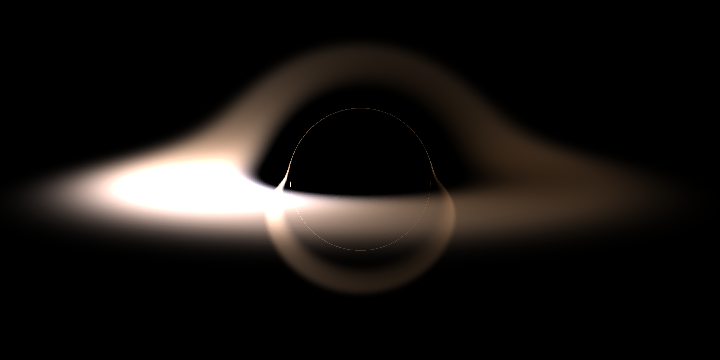
\includegraphics[width=\textwidth]{images/RelativisticAberationSageManifoldsindex.png}
\end{figure}

"Description of a bulk of space is encoded on boundary to bulk"


\end{frame}

\begin{frame}{Anti-de Sitter (AdS) space; "The Bulk"}

		\begin{figure}[!htb]
			\minipage{0.32\textwidth}
				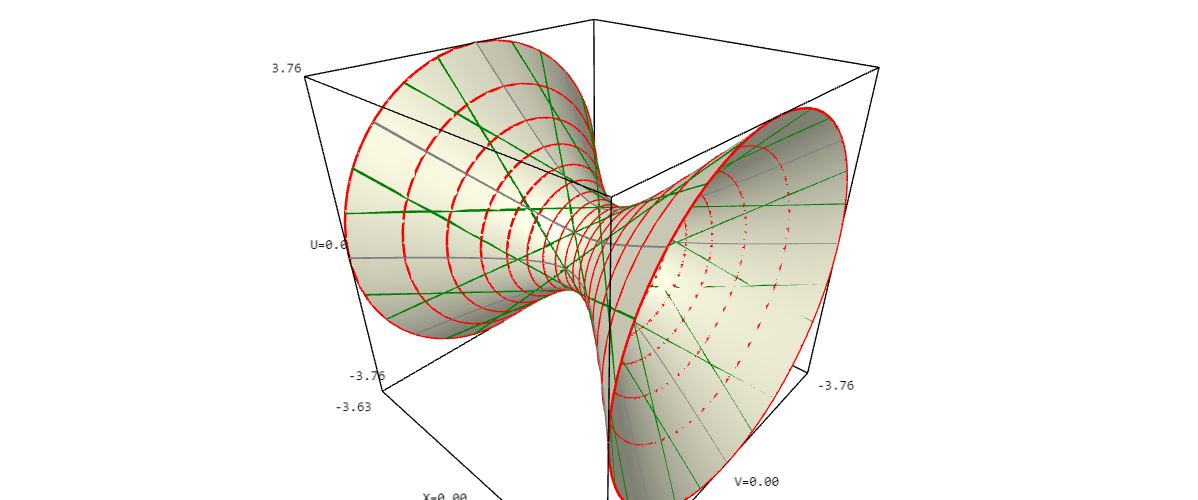
\includegraphics[width=1.5\linewidth]{images/AdSscreenshot1.png} 
			\endminipage\hfill
			\minipage{0.32\textwidth}
				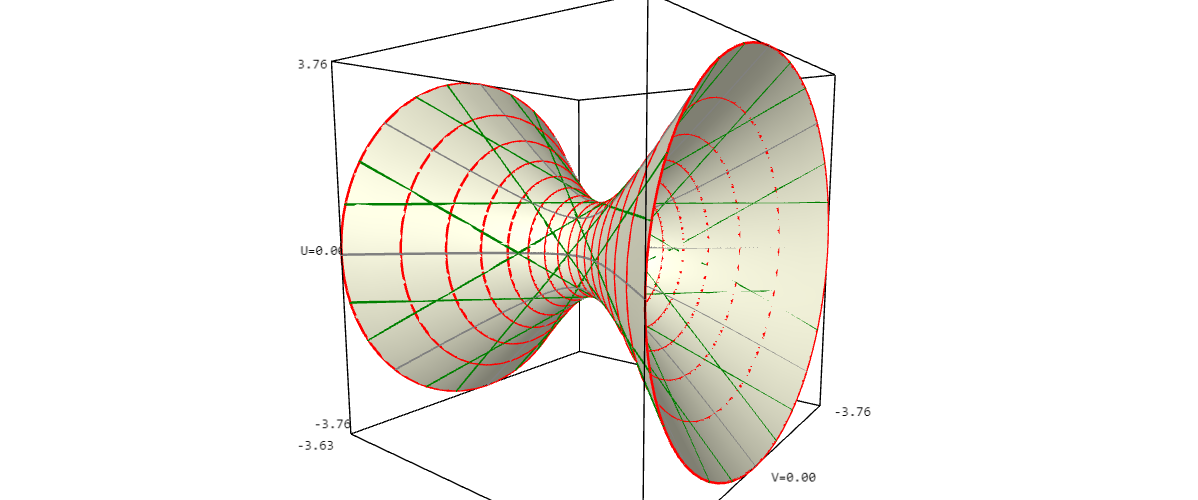
\includegraphics[width=1.5\linewidth]{images/AdSscreenshot2.png}
			\endminipage\hfill
			\minipage{0.32\textwidth}
				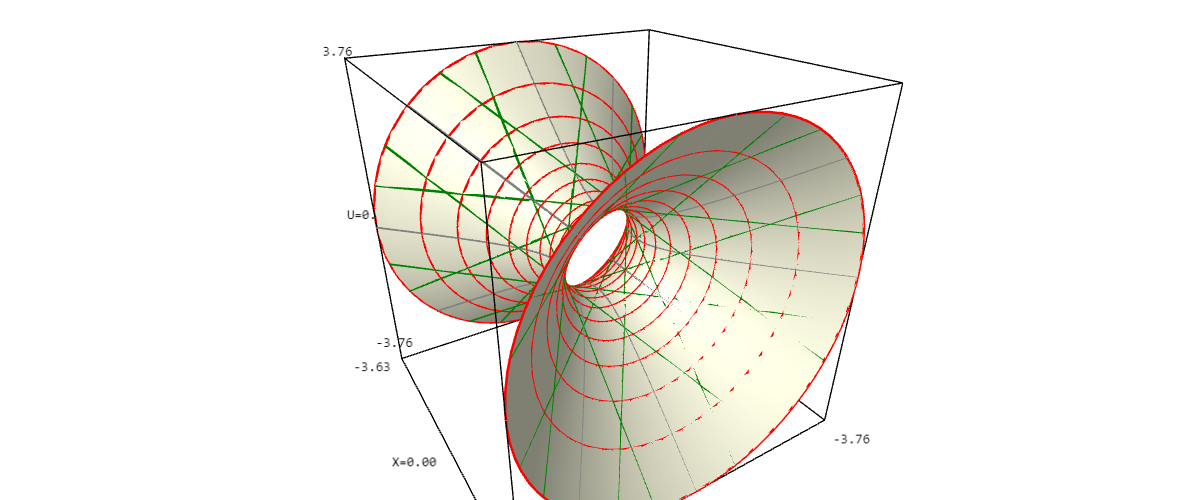
\includegraphics[width=1.5\linewidth]{images/AdSscreenshot3.png}
			\endminipage\hfill
		\end{figure}
\begin{equation*}
g = - dt^2 + \sum_{i=1}^4 dx_i^2
\end{equation*}

A coordinate patch for half-space:

\begin{equation*}
ds^2 = \frac{1}{y^2} \left( -dt^2 + dy^2 + \sum_i dx_i^2 \right)
\end{equation*}

\end{frame}

\begin{frame}{An example of the AdS/CFT correspondence}
\begin{equation*}
	\begin{array}{c c c}
		\fbox{$\substack{ \text{Quantum Field Theory} \\
			\text{in $d$ dimensions}}$}
		&  \underset{ \text{Holographic duality}}{ \overset{\text{AdS/CFT duality}}{\Longleftrightarrow} }
		& 
		\fbox{$\substack{ \text{String theory} \\
		\text{in $(d+1)$-dim.} \\
		\text{Anti-de Sitter space}}$}	
		\\
		\fbox{$\substack{ \mathcal{N} = 4 \, \text{Super Yang-Mills} \\
		\text{with gauge group in $SU(N)$}}$} 
	&
	&
	\fbox{$\substack{ \text{Type IIB String theory} \\
			\text{on $AdS_5 \times S_5$} }$}
	\\
	\end{array}
\end{equation*}

		\begin{figure}
	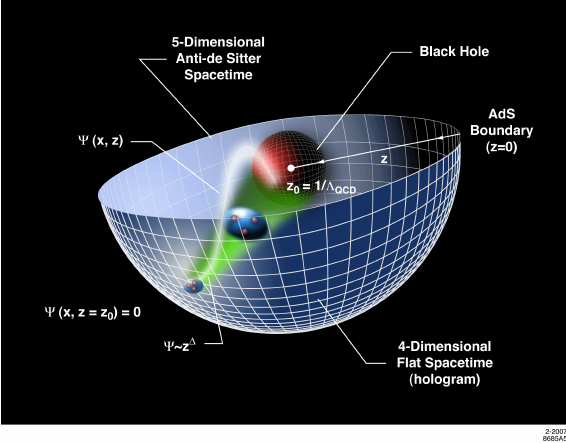
\includegraphics[width=0.7\textwidth]{images/Artists-conception-of-AdS-CFT-The-evolution-of-the-proton-at-different-length-scales-is.png}
\end{figure}

\end{frame}

\begin{frame}{Hints in the movie "Interstellar"}
		\begin{figure}
	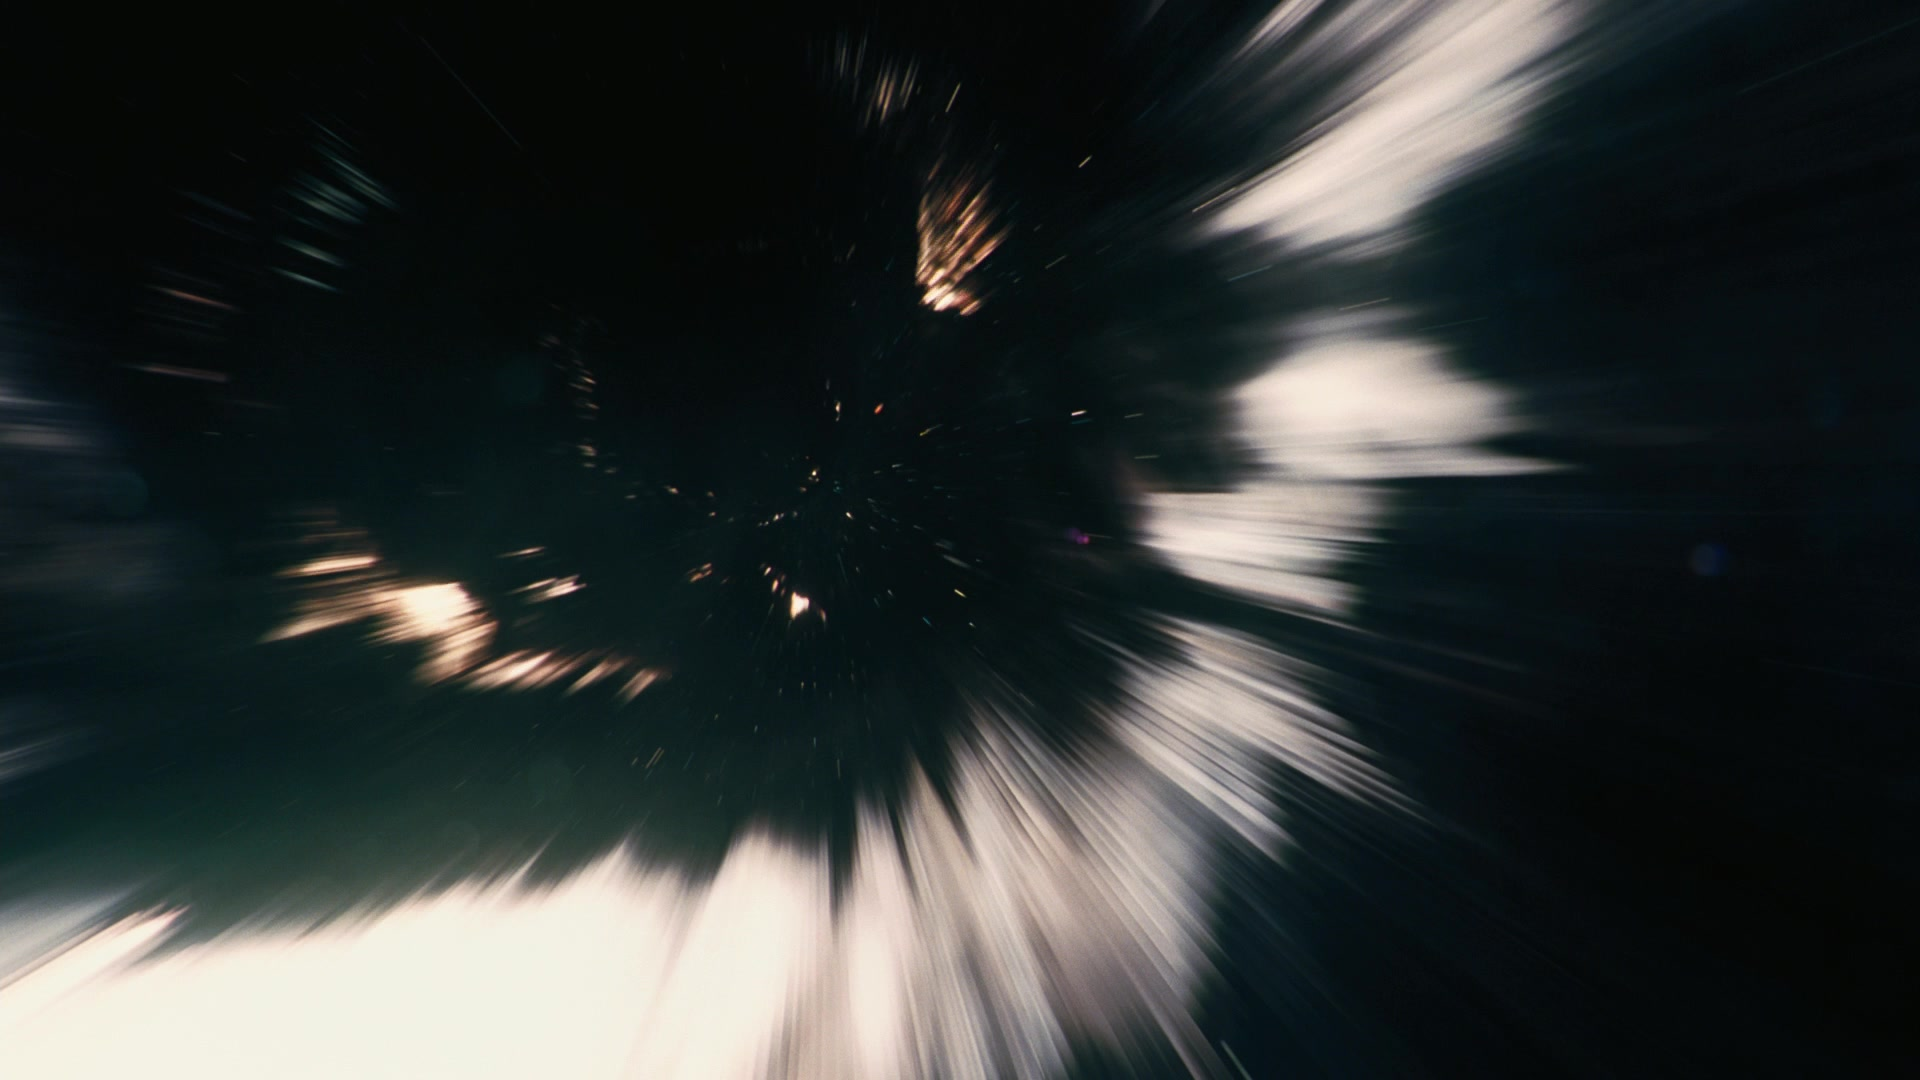
\includegraphics[width=\textwidth]{images/1198701.jpg}
\end{figure}
Controls won't work here. We're passing through the \textbf{bulk} - space beyond our 3 dims. All we can do is record and observe.

\end{frame}

\begin{frame}{Hints in the movie "Interstellar"}
		\begin{figure}[!htb]
	\minipage{0.42\textwidth}
	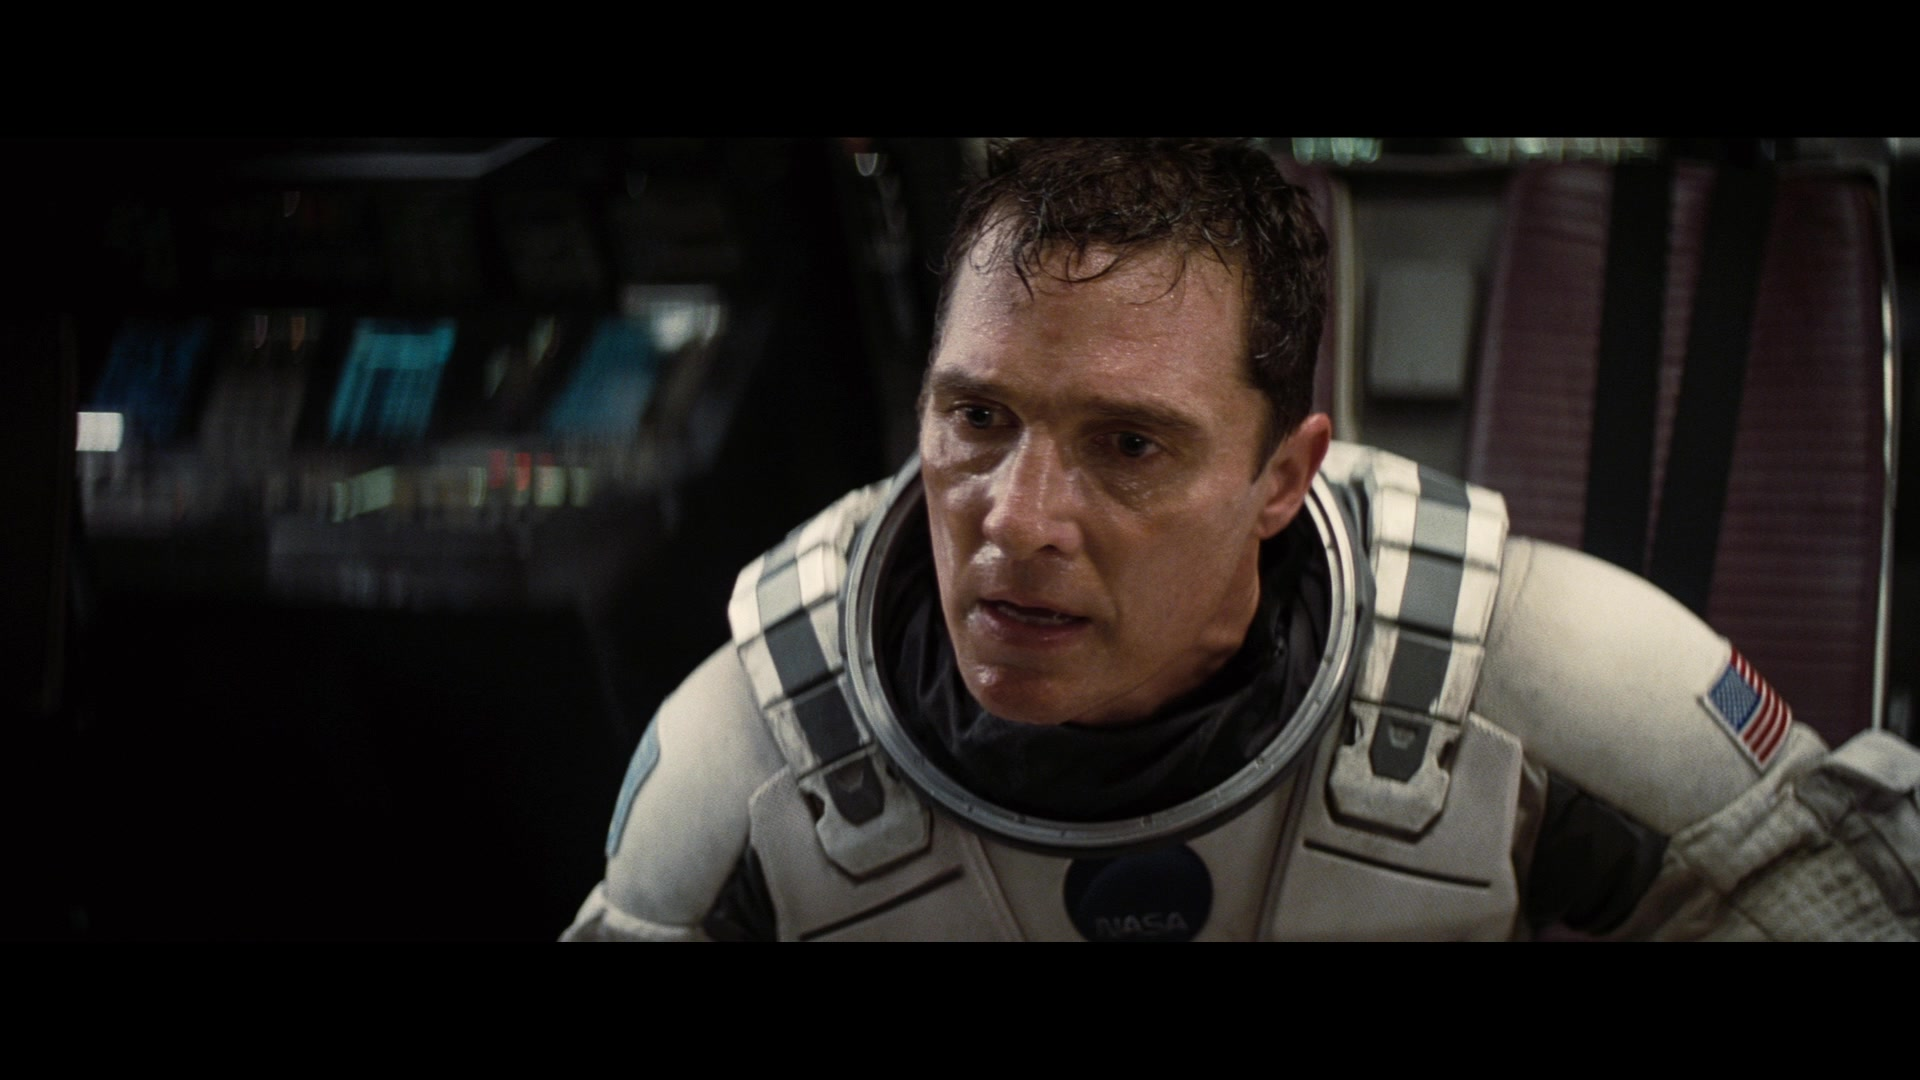
\includegraphics[width=1.5\linewidth]{images/1199149.jpg} 
	\endminipage\hfill
	\minipage{0.42\textwidth}
	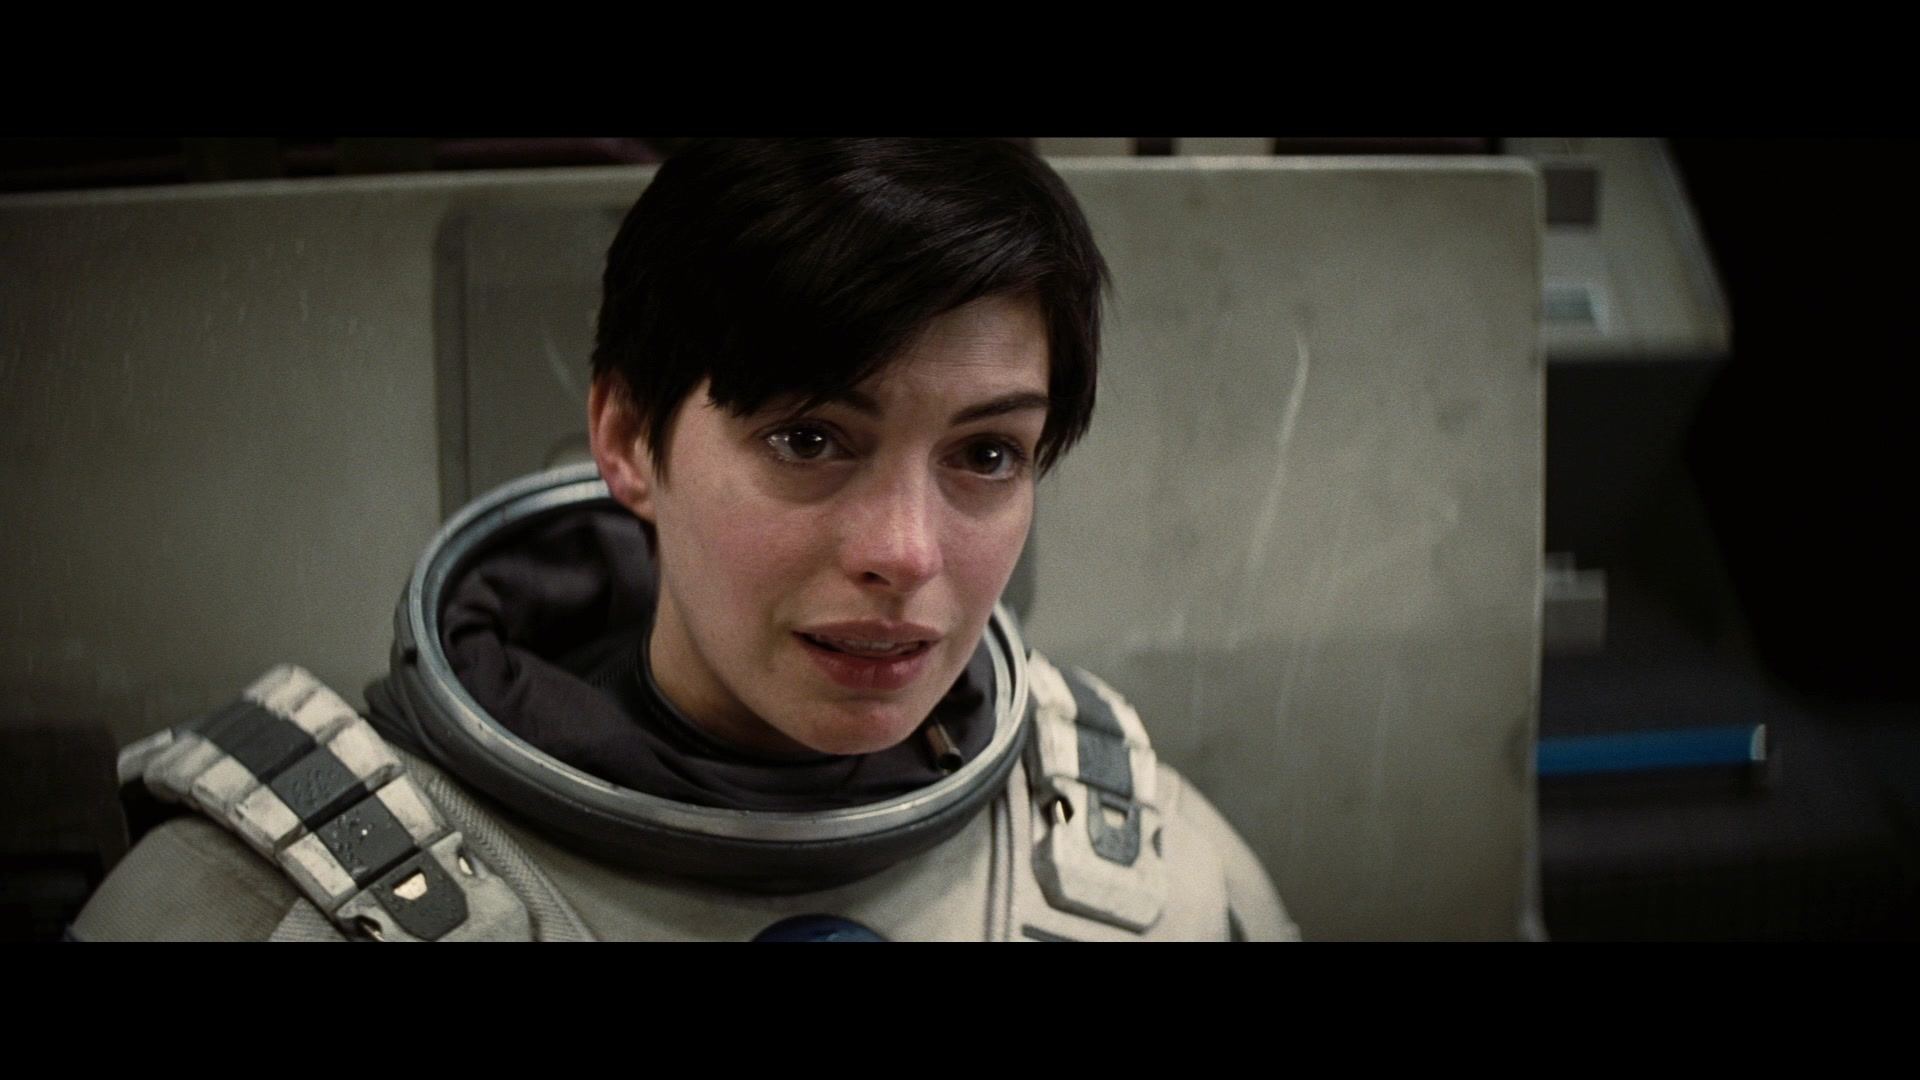
\includegraphics[width=1.5\linewidth]{images/1199158.jpg}
	\endminipage\hfill
\end{figure}
\emph{Cooper}: The beings who led us here. They communicate through gravity, right? ... \emph{Brand}: They are beings of 5 dimensions - to them time might be another physical dimension.
	
\end{frame}

\begin{frame}{Tesseract $\subset \, AdS_5$}
		\begin{figure}
			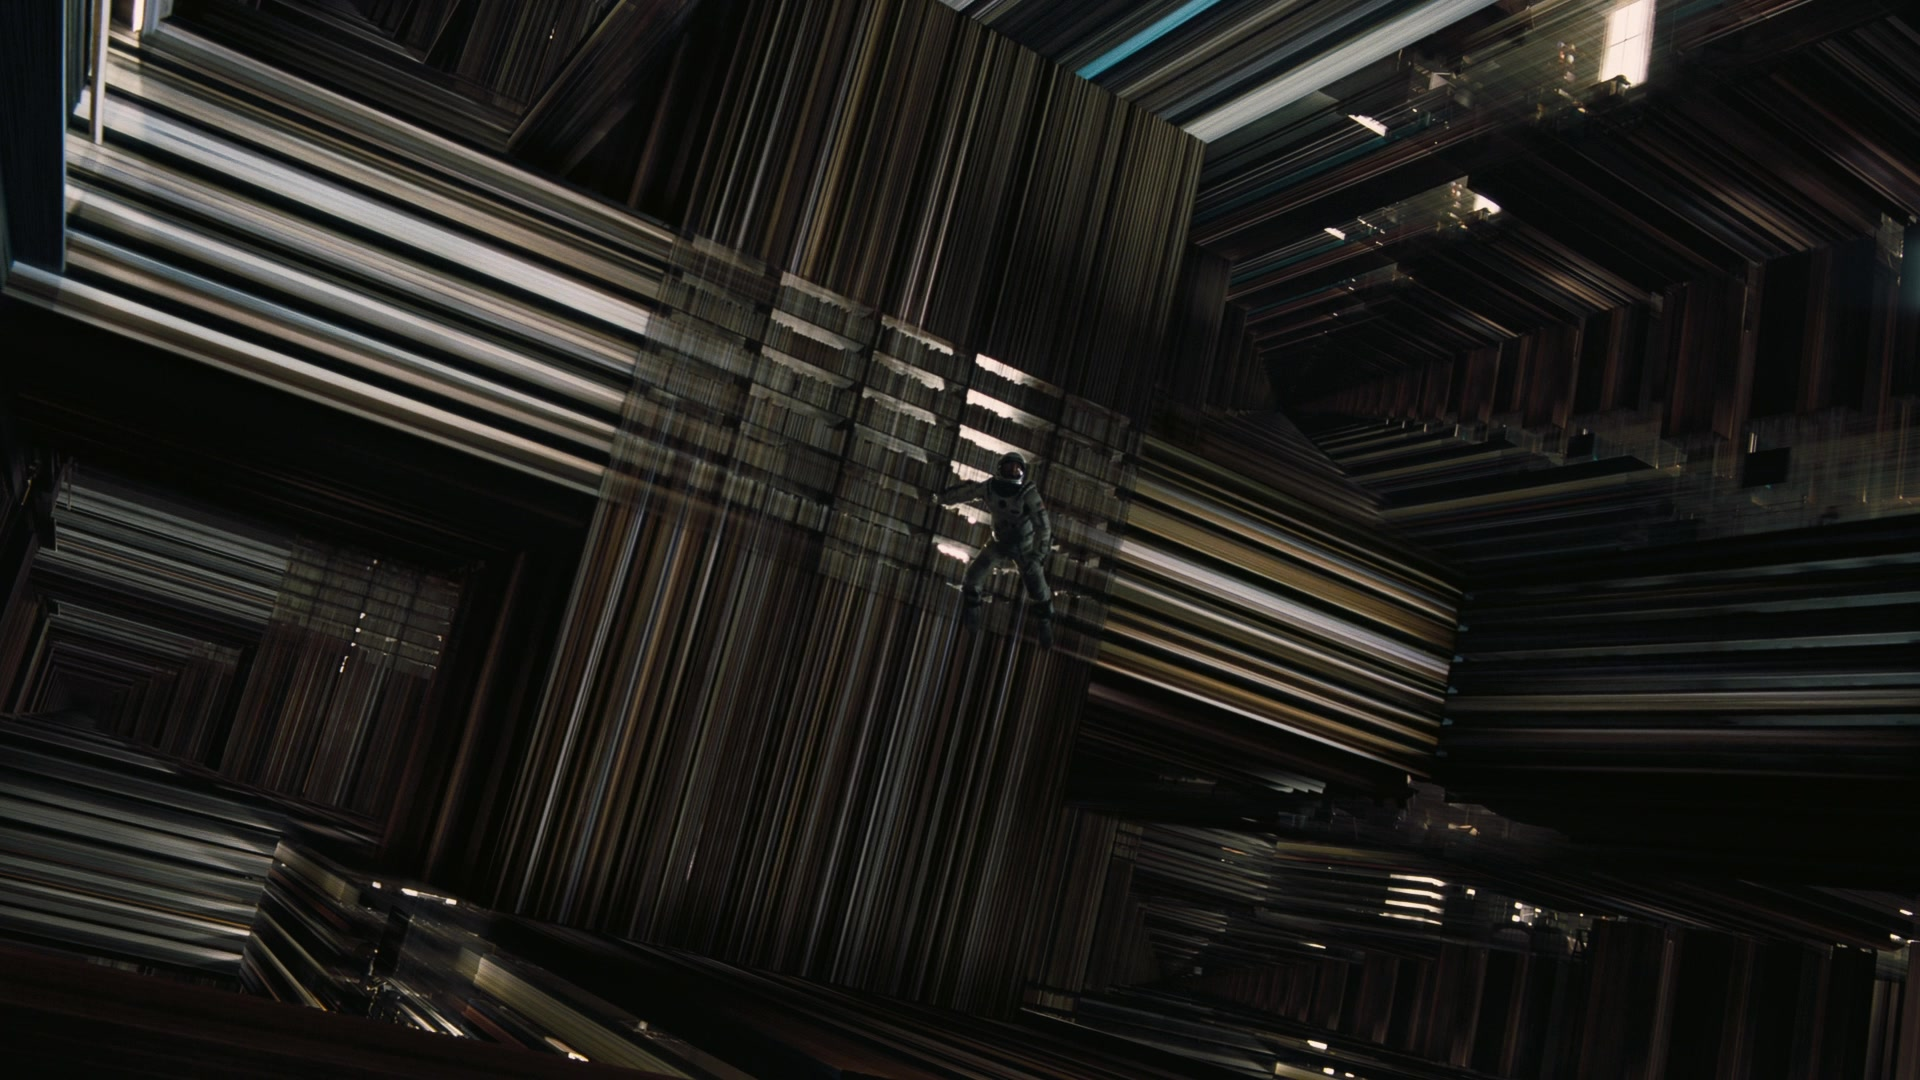
\includegraphics[width=\textwidth]{images/1201172.jpg}
		\end{figure}
\end{frame}

\begin{frame}{Messaging from the Tesseract $\subset$ bulk, 1}
	
	\begin{figure}
		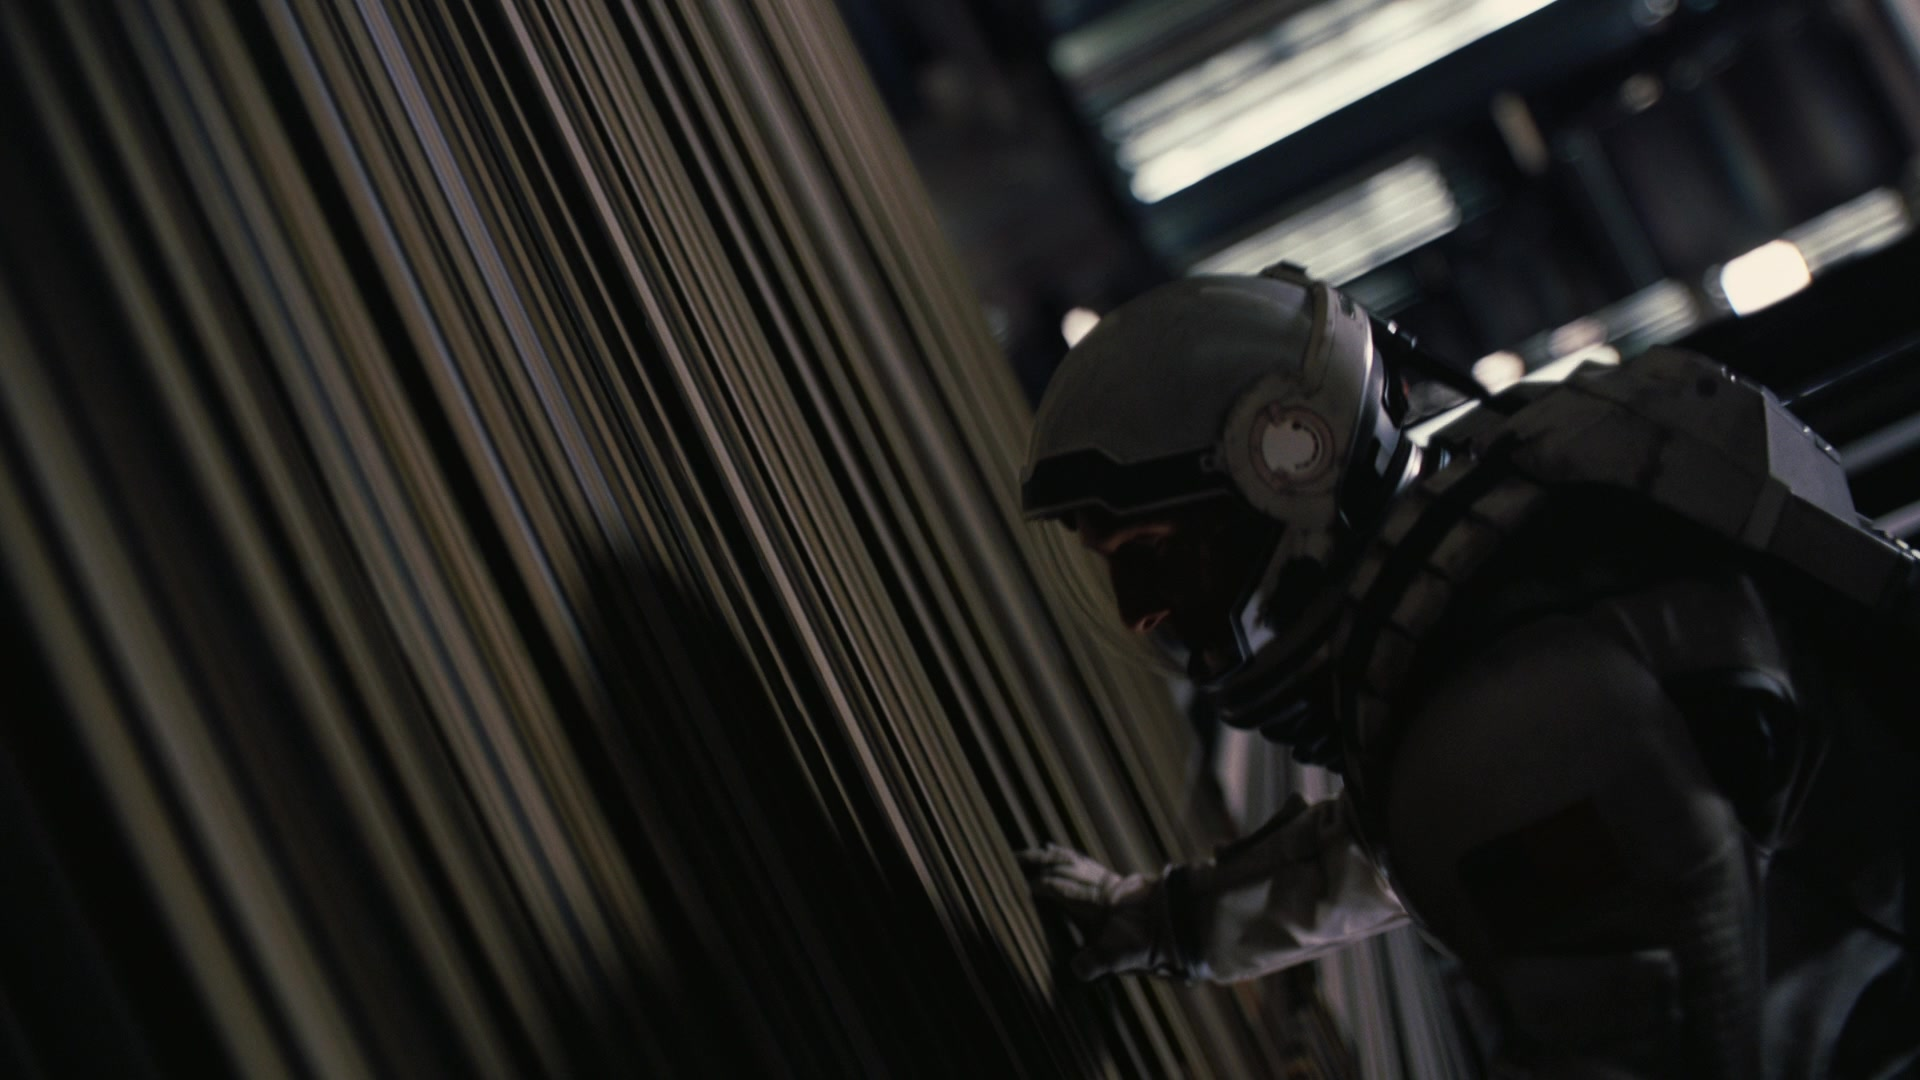
\includegraphics[width=\textwidth]{images/1201204.jpg}
	\end{figure}
	
	\emph{TARS}: You've seen that time is represented here as a physical dimension - you've worked out that you can exert a force across spacetime.
	
\end{frame}

\begin{frame}{Messaging from the Tesseract $\subset$ bulk, 2}
	
		\begin{figure}[!htb]
	\minipage{0.42\textwidth}
	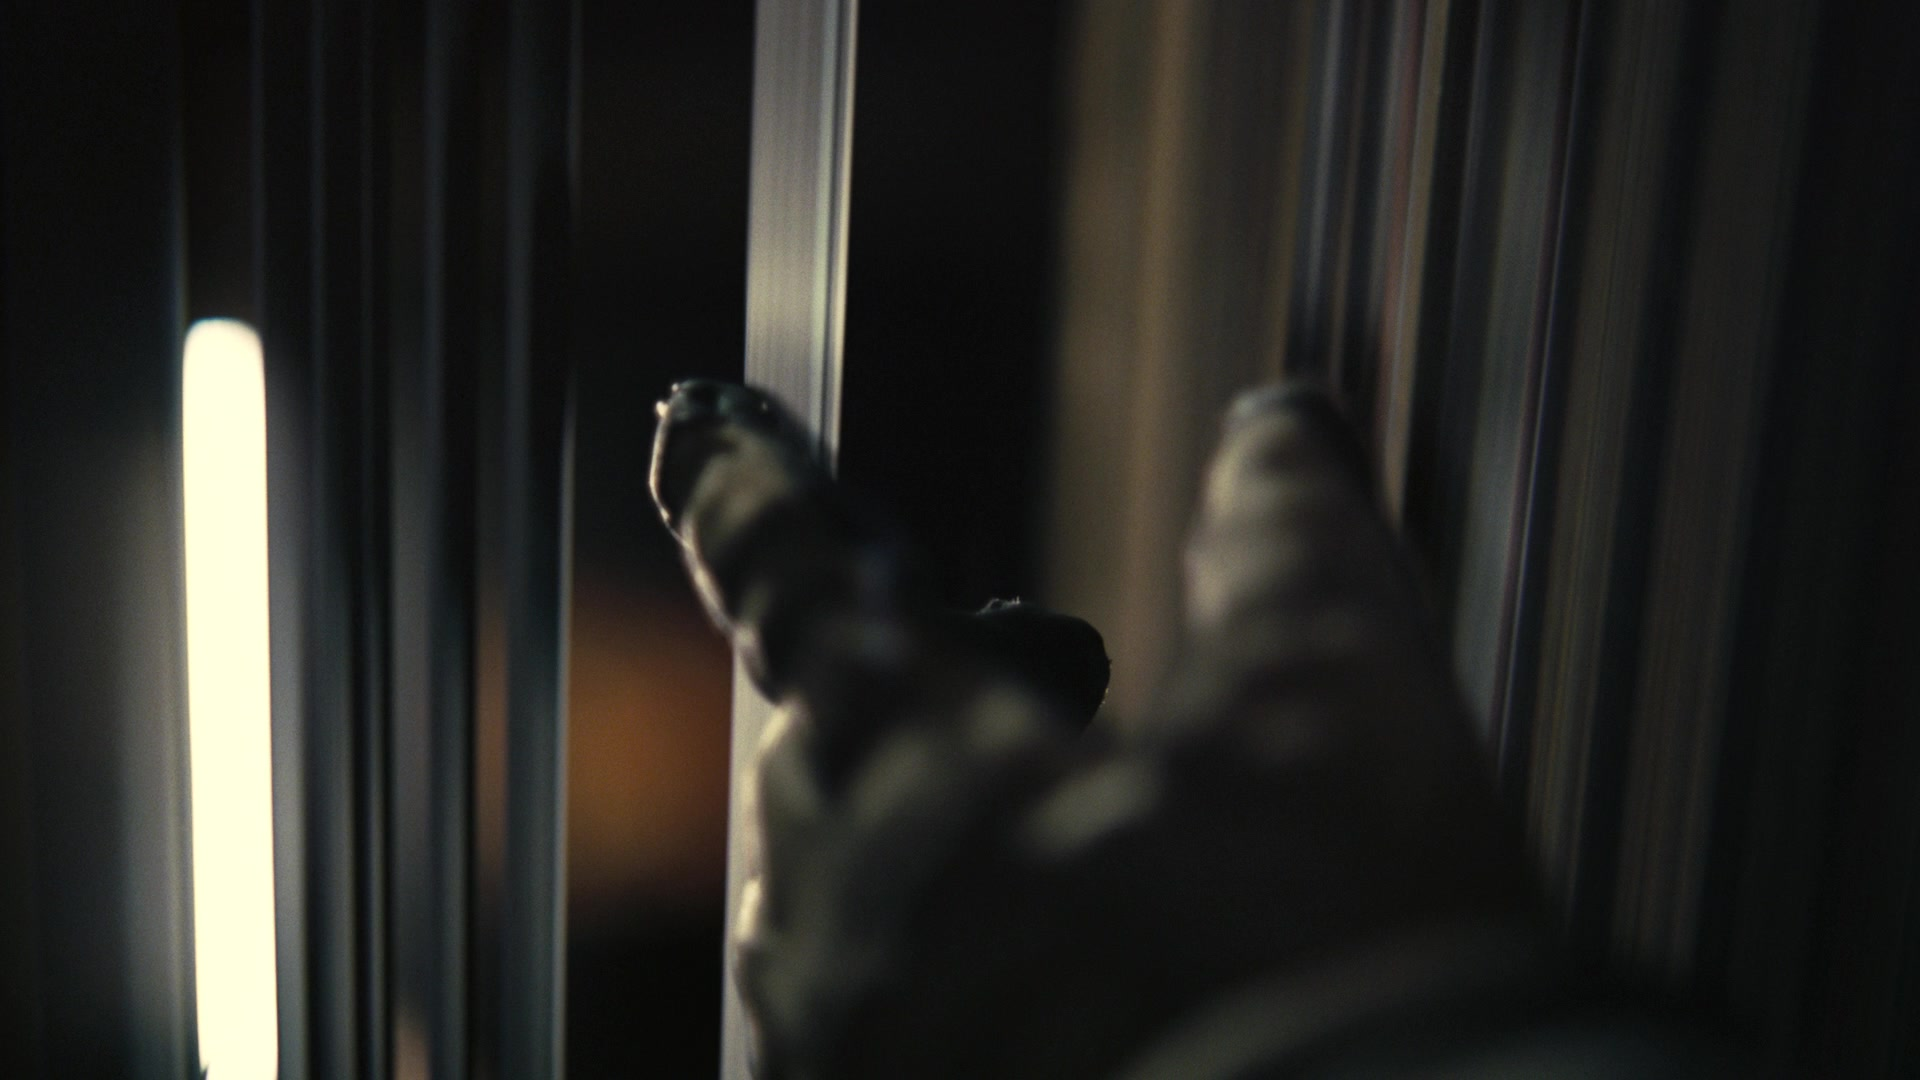
\includegraphics[width=1.5\linewidth]{images/1201440.jpg} 
	\endminipage\hfill
	\minipage{0.42\textwidth}
	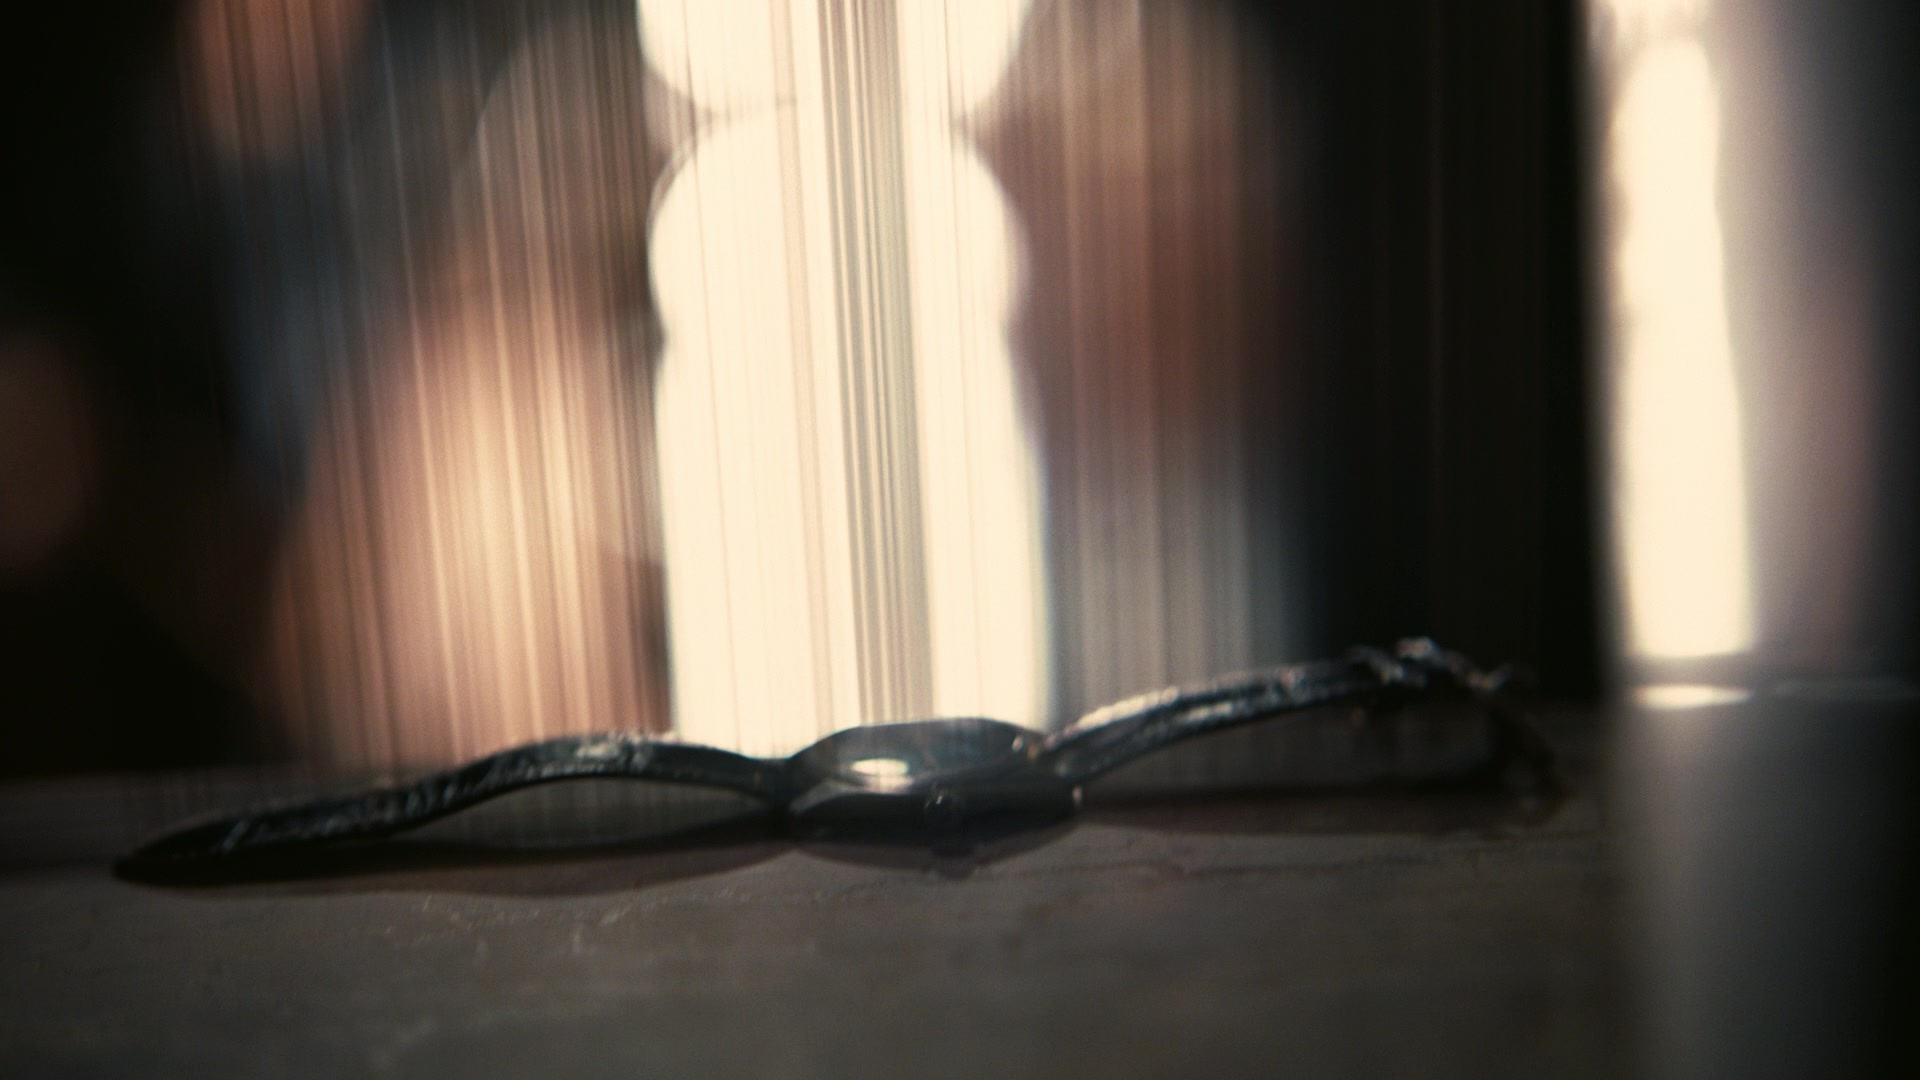
\includegraphics[width=1.5\linewidth]{images/1201442.jpg}
	\endminipage\hfill
\end{figure}

\emph{Cooper}: The watch. That's it. We encode the data into the movement of the second hand. TARS, translate the data into Morse and feed it to me.
	
\end{frame}



\begin{frame}{How did Cooper message Murph from the tesseract}

\begin{enumerate}
\item on $AdS_5$ metric
	\begin{itemize}
		\item gravity field
		\item Graviton (massless, spin-2 boson)
	\end{itemize}
\item EPR (Einstein-Podolsky-Rosen) pair
\begin{itemize}
	\item ER $=$ EPR
\end{itemize}
\end{enumerate}
\end{frame}

\begin{frame}{2014-}
2014-
\end{frame}

\begin{frame}{New directions for quantization}
\begin{enumerate}
\item Brane Quantization
\item BV QQuantization
\end{enumerate}
\end{frame}

\end{document}